\section{Introduzione}
In questo capitolo le sezioni \textbf{3.2} e \textbf{3.3} saranno introduttive agli elementi fondamentali che compongono l'architettura del modello proposto.\\
La sezione \textbf{3.4} descrive l'approccio sviluppato e come lo si è utilizzato.\\
La sezione \textbf{3.5}, infine, tratta dei risultati ottenuti.

\section{RNN}
Una TS è una \textbf{sequenza} di punti, ognuno di questi descrive il valore di una data variabile registrata in momenti diversi, solitamente, ad intervalli regolari.\\
Da questa definizione è facile intuire come i dati siano tra loro correlati, e non indipendenti, come spesso si assume in diverse tecniche di machine learning.\\
Gli approcci tradizionali quindi peccano da questo punto di vista, e l'analisi risulta difficile anche per il fatto che le serie possono avere lunghezze diverse in base al numero di osservazioni. Per una classica rete neurale, ad esempio, bisognerebbe adattare l'input layer in modo da allinearsi alla lunghezza delle TS e dovrebbe anche tenere conto della correlazione di osservazioni temporalmente vicine.\\
\\
Soluzioni provate in letteratura prevedono che si utilizzino diverse istanze della stessa rete neurale affinché ciascuna operi su porzioni diverse della stessa serie, per poi unire i risultati, riprendendo un po' l'idea di un ensemble.\\
Questa soluzione, per quanto semplice, non funziona bene con sequenze di dati, poiché, come detto, i dati sono tra loro correlati nel tempo: ogni valore nel tempo $t$ è legato al valore nel tempo $t-1$. Con questa soluzione le reti si addestrano su sottosequenze indipendenti della stessa TS, ma si perdono le correlazioni esistenti.\\
\\
Il concetto, dunque, è quello di non perdere le informazioni del passato. Questo approccio ricorda molto quello umano, che non lascia che i pensieri vengano generati partendo dal nulla, ma che siano determinati a partire dal passato, cioé da quello che si conosce. Una \textbf{rete neurale ricorrente} (Recurrent Neural Network, RNN) è fa proprio questo: rispetto una rete neurale consueta non ha solamente archi che confluiscono in un'unica direzione, dall'input all'output, ma ne ha altri che possono "tornare indietro".\\
In questo modo viene risolto il problema di dover tenere memoria delle sottosequenze analizzate nel passato e di prendere decisioni in funzione di esse.\\
Una RNN usa l'output del \textbf{layer ricorrente} come input dello stesso per un certo numero di iterazioni (ripetizioni). Tra una ripetizione e l'altra, il risultato degli input precedenti va a condizionare quelli successivi, così da tenere la memoria della sottosequenza di dati visti in precedenza e conservare le correlazioni.\\
I pesi che evolvono nel tempo all'interno del layer ricorrente formano il cosiddetto \textit{hidden state}, o stato nascosto. Questa tecnica viene chiamata \textbf{parameter sharing}.\\
La dimensione del layer ricorrente è fissata ed andrà a determinare le dimensioni dell'input e dell'output, e corrisponderà alla dimensione della sottosequenza che si desidera analizzare ad ogni iterazione.
\begin{figure}[H]
	\centering
	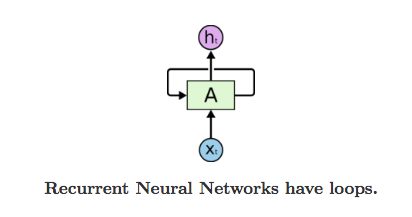
\includegraphics[width=\linewidth]{rnn.png}
	\caption{L'architettura base di una RNN}
	\label{fig:rnn}
\end{figure}
E' molto comune dare una rappresentazione \textit{unrolled} della rete per poterla ricondurre ad una rete neurale classica e comprenderne il funzionamento nel dettaglio.
\begin{figure}[H]
	\centering
	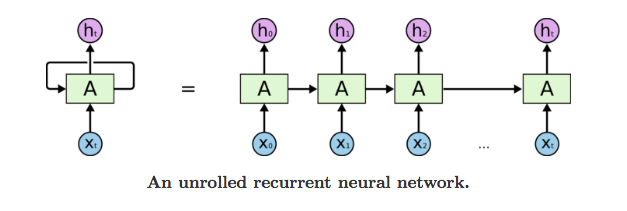
\includegraphics[width=\linewidth]{rnn_unrolled.png}
	\caption{La rappresentazione unrolled di una RNN}
	\label{fig:rnn_unrolled}
\end{figure}

Chiaramente, è possibile rendere più profonda una RNN, ed esistono diversi modi per farlo:
\begin{itemize}
	\item Aggiungere dei layer nascosti ricorrenti. Detta soluzione \textbf{stacked};
	\item Rendere il layer ricorrente una sotto-rete profonda;
	\item Aggiungere dei layer tra l'input e quello ricorrente;
	\item Aggiungere dei layer tra il ricorrente e l'output;
\end{itemize}

\subsection{LSTM}
Come evidenziato da Bengio et al.\cite{long_term}, il modello standard di RNN nella pratica soffre di un problema relativo alle \textbf{long-term dependencies}: man mano che la rete compie un alto numero di ripetizioni del layer ricorrente, le caratteristiche apprese dalla prime iterazioni iniziano a diventare meno rilevanti, quasi come se la rete iniziasse a dimenticare cosa ha fatto nel passato non recente. In molti casi è importante mantenere le informazioni che risalgono ad un passato meno recente.\\
\\
Per risolvere questo problema, Hochreiter et al.\cite{lstm} hanno presentato la più applicata implementazione di RNN, ovvero le reti \textbf{LSTM, Long Short Term Memory}.\\
Il layer ricorrente di una LSTM segue una precisa struttura, ed è chiamato \textbf{cella LSTM}. Mentre nelle RNN standard i layer ricorrenti sono composti da neuroni che applicano una qualsiasi funzione di attivazione, un layer LSTM è invece composto da quattro sotto-layer, che applicano delle funzioni più complesse.
\begin{figure}[H]
	\centering
	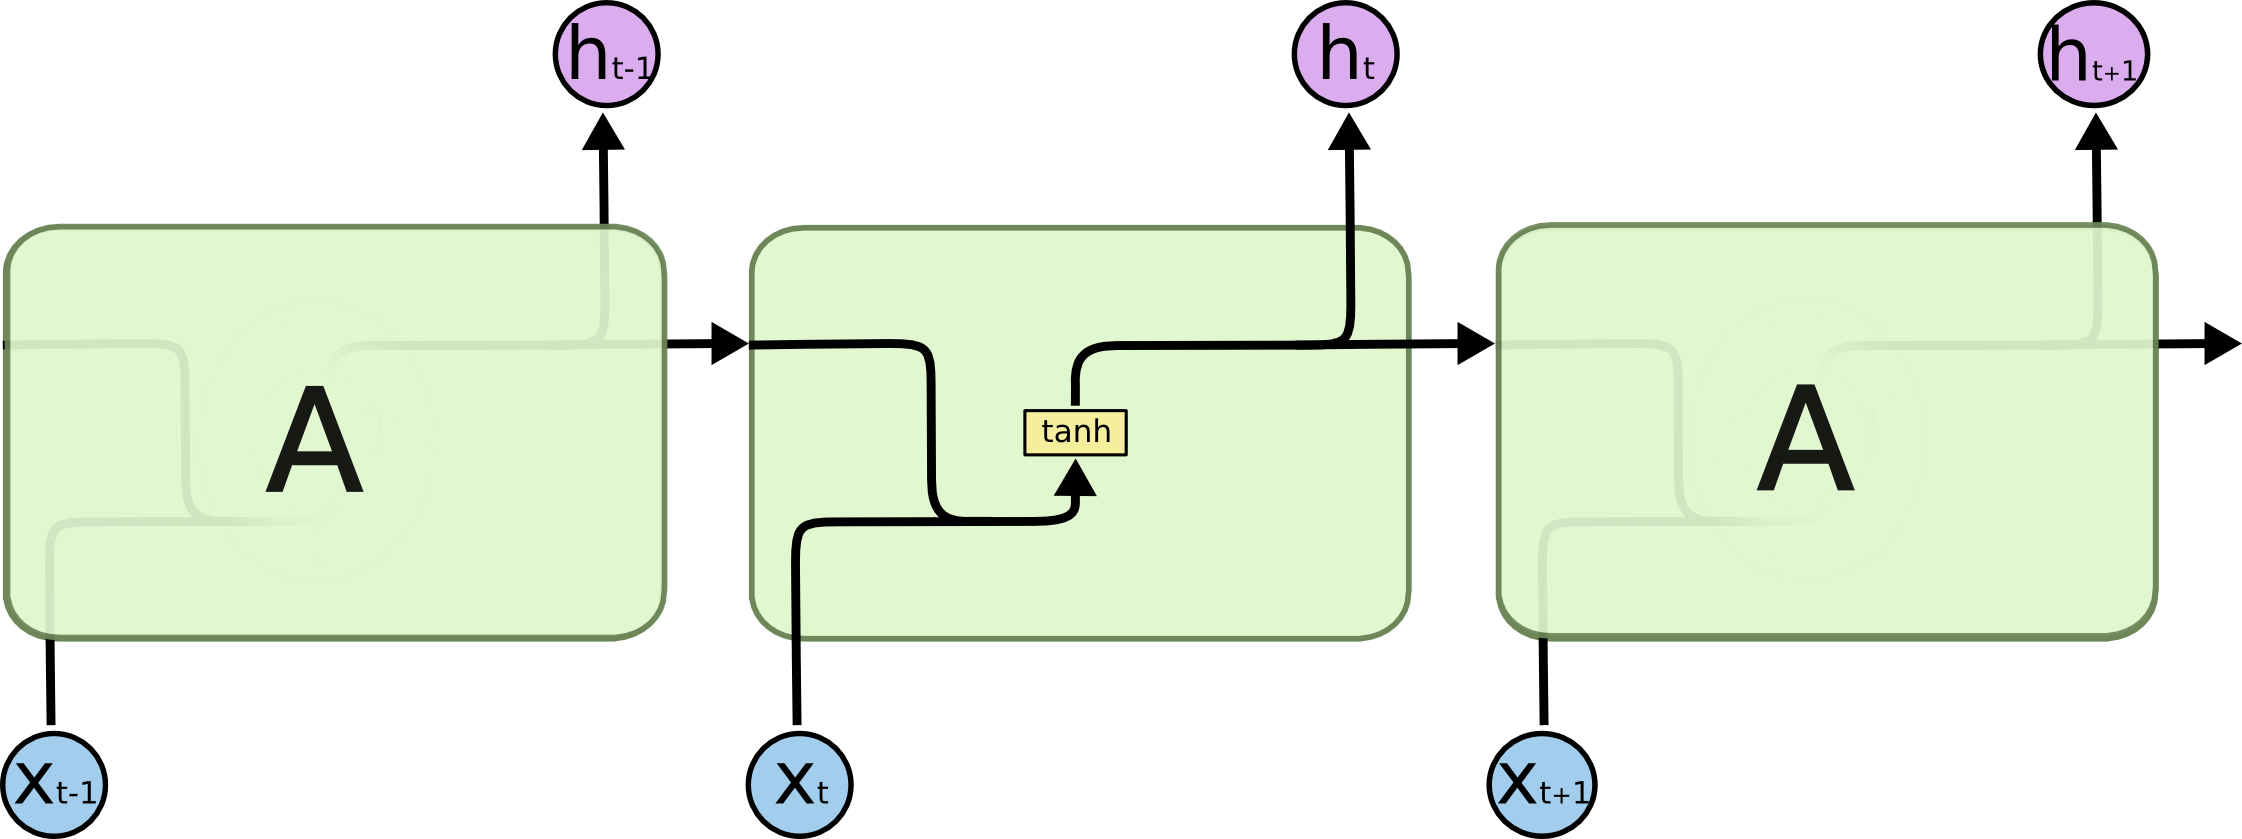
\includegraphics[width=\linewidth]{rnn_2.png}
	\caption{RNN unrolled standard. Nell'esempio viene usata la funzione di attivazione tangente iperbolica.}
	\label{fig:rnn_2}
\end{figure}
\begin{figure}[H]
	\centering
	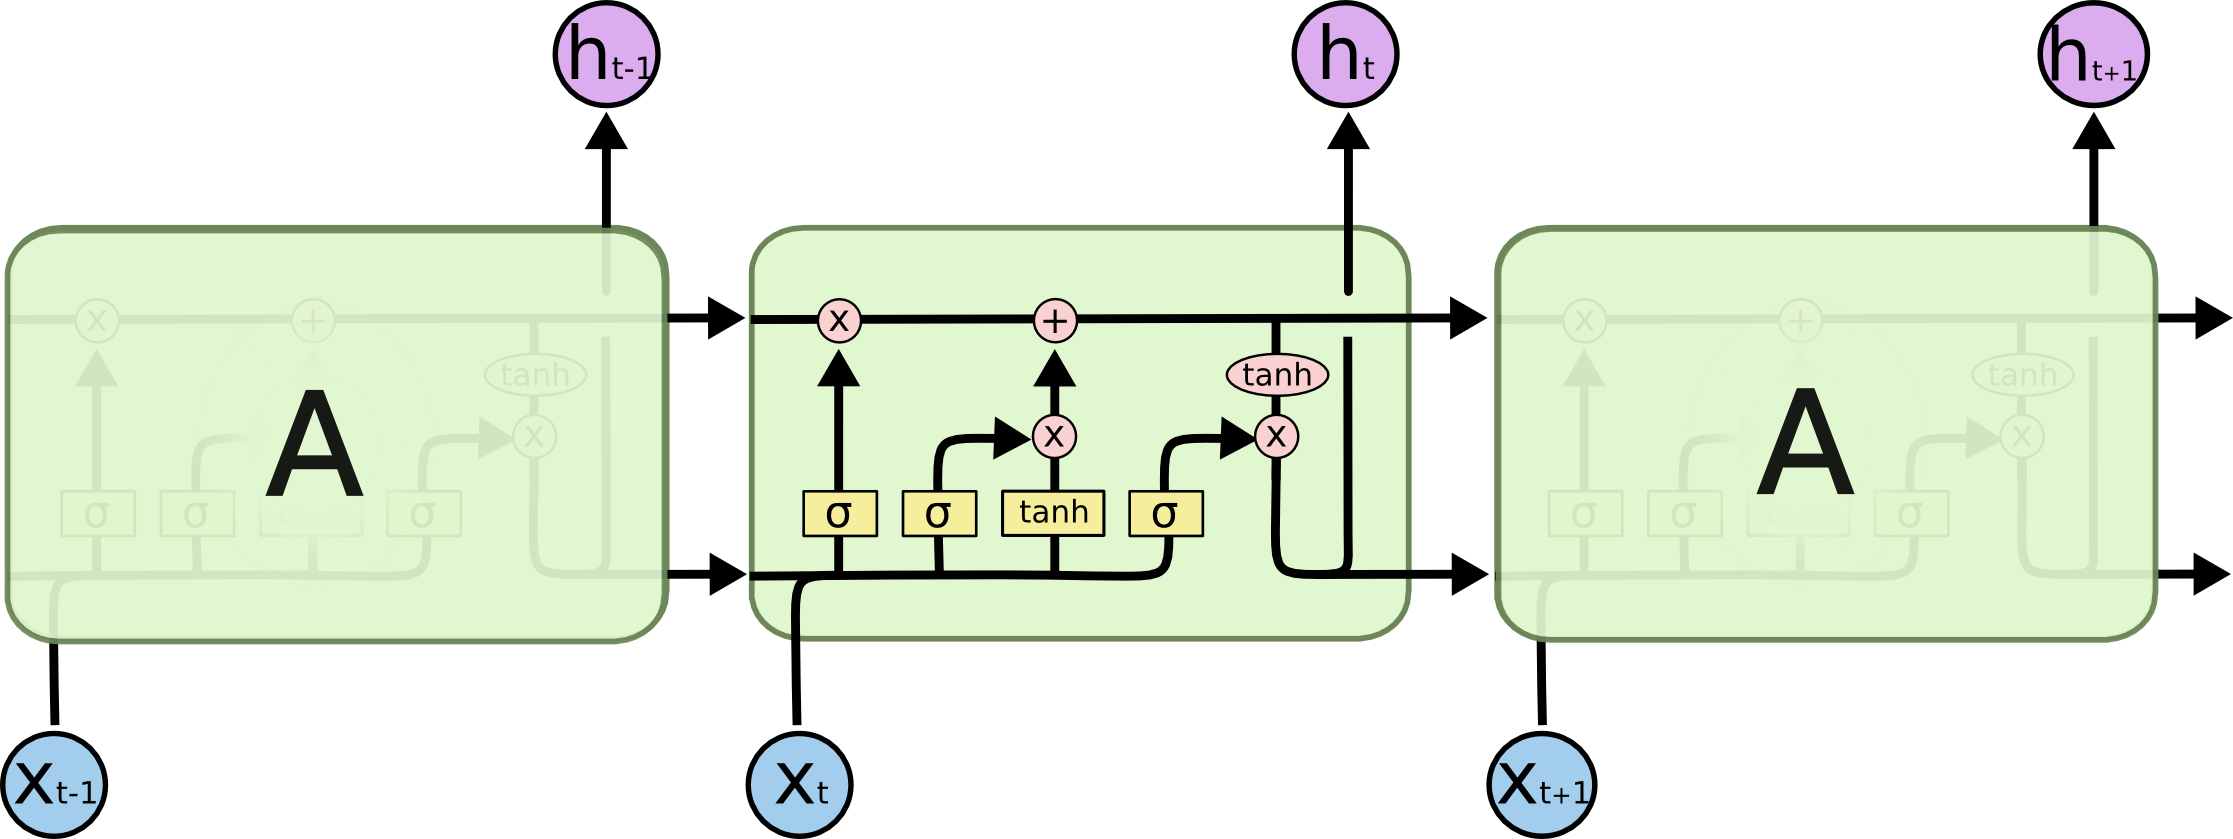
\includegraphics[width=\linewidth]{lstm.png}
	\caption{LSTM unrolled. I rettangoli gialli sono i quattro sotto-layer, di cui tre di essi applicano la semplice sigmoide, mentre l'altro la tangente iperbolica, mentre le figure rosa sono operazioni su vettori semplici.}
	\label{fig:lstm}
\end{figure}

La linea superiore della cella trasporta l'output superiore della cella precedente direttamente alla cella successiva, a meno di alcune operazioni lineari. Serve a mandare in avanti la conoscenza del passato senza modificarla troppo.\\
\\
La cella LSTM non segue necessariamente lo schema suddetto, ed esistono altre varianti, tutte accomunate dall'idea di avere un flusso che preservi le long-term dependencies.\\
La \textbf{hidden size}, cioè dimensione dell'hidden state, determina la dimensione dei quattro sotto-layer, ovvero il numero dei loro neuroni. Il numero totale dei neuroni presenti in una LSTM è allora dato dalla $hidden size * 4$. Tipicamente, \textbf{al crescere della hidden size cresce anche la capacità di memorizzazione della LSTM}.

\section{Autoencoder}
Un \textbf{autoencoder} è una tipologia di rete neurale che cerca di apprendere una rappresentazione "compressa" di un input, per poi tentare di ricostruirlo correttamente come output.\\
Nonostante questo possa sembrare confusionario ed inutile, una rete che impara una versione compressa dei dati si presta in maniera ottimale a risolvere una serie di task che altrimenti non avrebbero soluzioni adeguate. Sostanzialmente un autoencoder è un metodo per ottenere una rappresentazione di \textbf{dimensione ridotta} di un input di dimensionalità superiore.\\
\\
Un autoencoder prende i dati dall'input layer e li trasforma in una rappresentazione interna, detta \textbf{codifica} o \textbf{vettore latente}. Questa rappresentazione è ottima quando l'autoencoder con essa è in grado di ricostruire correttamente l'input, infatti il training di questa particolare rete consiste nel tentare di fornire un vettore latente ottimale per ciascun input.\\
Lo scopo finale non è quello di ricostruire perfettamente l'input (sarebbe abbastanza inutile) ma quello di estrarre dagli input \textbf{questo vettore latente ottimale che conterrà le loro principali caratteristiche}. In altre parole, si pone di estrarre feature rilevanti dall'input.\\
La compressione e la decompressione vengono effettuate attraverso delle funzioni che imparano automaticamente, senza l'ausilio dell'uomo (\textbf{unsupervised}), dai sample di un training set. In quasi tutti i contesti in cui sono usati gli autoencoder, le funzioni di compressione e decompressione sono implementare con reti neurali (nel nostro caso \textbf{LSTM}).\\
\\
Per compiere la ricostruzione è necessario che input e output layer siano della stessa dimensione, tuttavia, al fine di permettere alla rete di estrarre le feature dagli input, il layer nascosto che genera la codifica, detto \textbf{coding layer}, dovrà necessariamente essere di dimensione minore degli input e output layer. Si parla di autoencoder \textbf{undercomplete}.\\
\\
Come detto un autoencoder è sempre composto da:
\begin{itemize}
	\item Un \textbf{encoder}, solitamente una rete neurale che riduce l'input nella codifica. Anche detta \textit{rete ricognitiva};
	\item Un \textbf{decoder}, solitamente una rete neurale che ricostruisce l'input dell'encoder a partire dalla codifica. Anche detta \textit{rete generativa};
\end{itemize}
Encoder e decoder sono simmetrici rispetto al coding layer.
\begin{figure}[H]
	\centering
	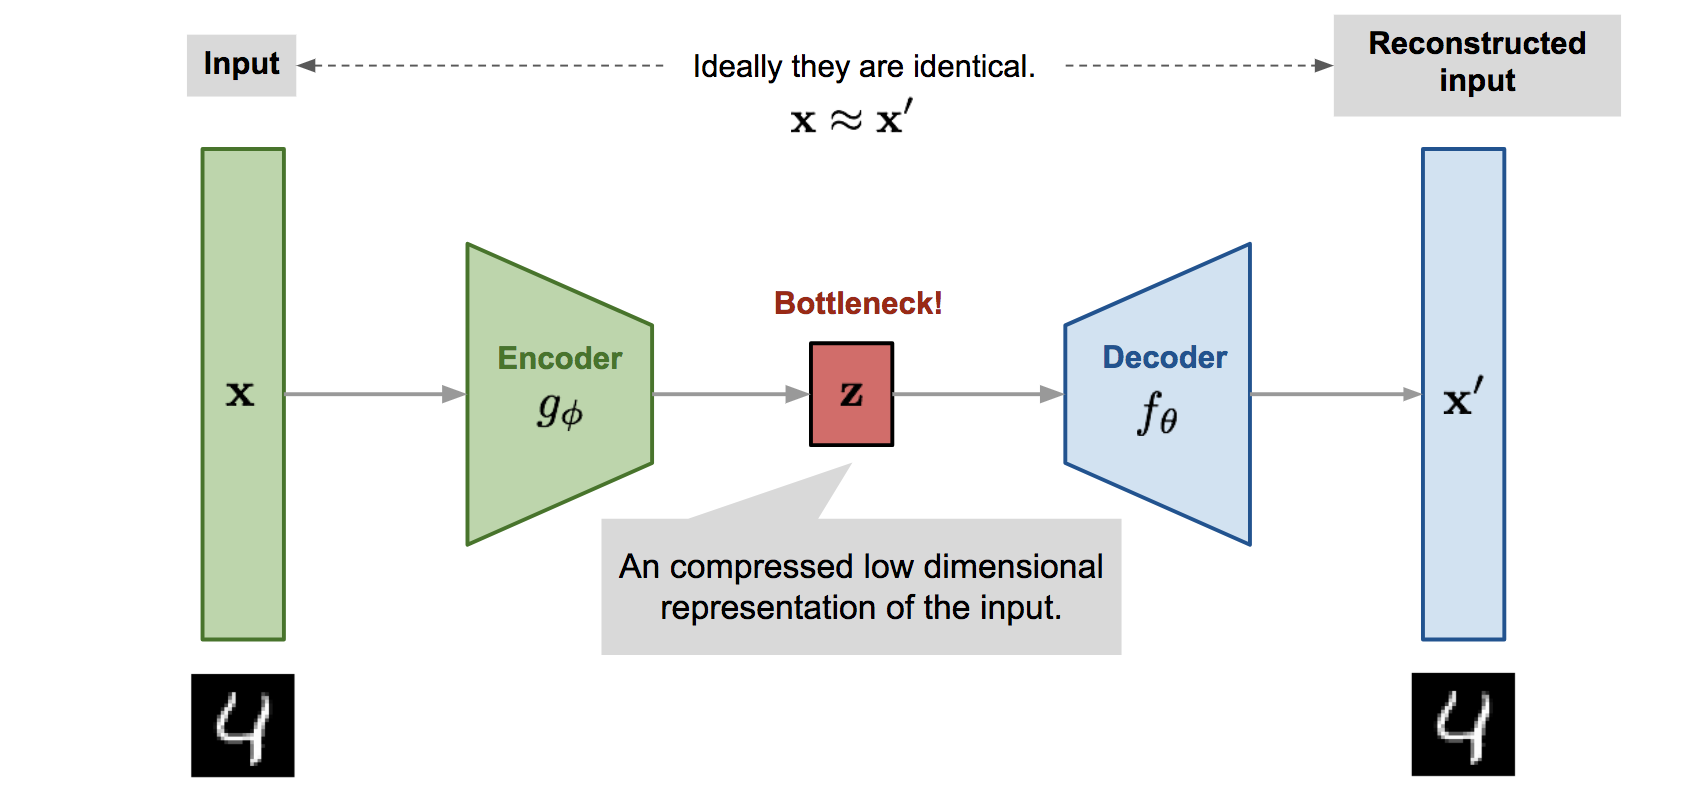
\includegraphics[width=\linewidth]{autoencoder.png}
	\caption{Schema di un autoencoder.}
	\label{fig:autoencoder}
\end{figure}

Gli autoencoder sono usati principalmente per fare \textbf{dimensionality reduction}, dato che la codifica è una rappresentazione ridotta di ogni input, ma anche \textbf{generazione di sample}, ovvero generare nuovi dati a partire da codifiche arbitrarie.\\
\\
Come una qualsiasi altra rete neurale, gli autoencoder possono essere resi più profondi aggiungendo layer nascosti, sia dal lato dell'encoder che dal lato del decoder. In tal caso si parla di \textbf{autoencoder stacked}.\\
In generale, un maggior livello di profondità permette alla rete di comprendere pattern più complessi, tuttavia una profondità troppo alta rende il rischio di overfitting più alto.

\subsection{Variational Autoencoders}
Come i tradizionali autoencoder, i \textbf{Variational Autoencoders} (VAEs) cercano di ricostruire gli input utilizzando un encoder e un decoder. Anche in questo caso, l'output dell'encoder è una rappresentazione compressa dell'input, e il decoder impara a ricostruire l'input iniziale prendendo come punto di partenza la rappresentazione compressa generata dall'encoder.\\
Ciò che rende particolare questa tipologia di autoencoder è che il modello prevede un \textbf{approccio probabilistico} per descrivere le osservazioni nello spazio latente.\\
Anziché costruire un autoencoder il cui output è un singolo valore per ogni attributo del vettore dei fattori latenti, questo viene formulato in maniera tale da descrivere una \textbf{distribuzione di probabilità} per ogni attributo latente, tipicamente una distribuzione normale.\\
Costruendo l'encoder in questo modo otteniamo un range di possibili valori (la distribuzione, appunto), e l'esito è quello di forzare il modello a rappresentare l'input in uno spazio latente continuo e regolare rispetto ai valori iniziali. Per ogni campione della \textbf{distribuzione latente} ci aspettiamo che il decoder sia in grado di ricostruire l'input. I valori che sono vicini uno all'altro nello spazio latente in questo modo vengono ricostruiti in maniera simile. 

\section{Modello proposto}
\subsection{Architettura e motivazione}
Il modello proposto è composto da quattro componenti fondamentali:
\begin{itemize}
	\item Il primo componente è l'\textbf{encoder} costituito da una rete \textbf{Stacked LSTM}. Questa prende in input un vettore che descrive una TS;
	\item Successivamente, vi è una componente adibita al mappare l'\textbf{hidden vector} ottenuto dall'encoder in un vettore dei \textbf{fattori latenti}. In questo layer viene effettuato il train dei punti nello spazio latente per avere media nulla e varianza unitaria (il perché è discusso nella prossima sezione relativa al training);
	\item La componente successiva deve fare il processo inverso al precedente, cioè mappare il vettore latente nel vettore input per il decoder;
	\item l'ultima componente è il \textbf{decoder} che è una rete Stacked LSTM speculare a quella dell'encoder che prende il singolo vettore ricevuto e lo mappa in una sequenza di vettori in output, cioè cerca di ricostruire gli input.
\end{itemize}

L'idea dietro il modello è quella che, attraverso le LSTM, si possano ottenere le feature più significative delle serie temporali in input.\\
Se il modello converge vuol dire che il vettore latente è sufficientemente preciso nel ricostruire l'input iniziale. Il vettore latente che si ottiene viene poi utilizzato per effettuare il clustering con k-means.\\
\\
Il cuore del modello è sicuramente nel'utilizzo delle LSTM: nello studio delle serie temporali, le LSTM sono attualmente considerate il miglior "strumento" per ottenere buoni risultati nella maggior parte dei casi. Il problema delle serie temporali è infatti quello di avere molto rumore e di nascondere influenze nascoste nei dati.\\
Modelli troppo semplici non si comportano adeguatamente su questo tipo di dati, mentre le LSTM riescono a superare questi problemi, ma anche quelli relativi agli andamenti irregolari, come ad esempio l'avere linearità e non linearità nella stessa serie temporale.

\subsection{Training e iperparametri}
L'obiettivo del training è quello di imparare la funzione di identità in maniera tale che la sequenza dei vettori di input e output sia simile.\\ 
Come detto, è stato usato un approccio probabilistico: l'obiettivo è ricavare i parametri della distribuzione normale dell'hidden vector, cioè $\mu$ e $\sigma$, cercando di minimizzare il \textbf{logaritmo di verosimiglianza} dell'input sotto questa distribuzione.\\
La scelta di imporre la distribuzione normale è stata dettata sia dalla letteratura disponibile, che consiglia questa distribuzione, ma anche del fatto che altrimenti non sarebbe stato possibile utilizzare la tecnica della discesa stocastica del gradiente nella variante \textbf{Adam} (ADAptive Moment estimation), anch'esso in letteratura ritenuto il miglior optimizer per questo tipo di problemi.
\\
Durante il training è stato necessario lavorare sui tanti \textbf{iperparametri} della rete. I principali, sui quali si è data maggiore attenzione, sono:
\begin{itemize}
	\item \textbf{Number of layers}, indicante il numero di LSTM messe in stack. E' stato scelto 2 per tutti i dataset, per evitare di dare troppa complessità al modello;
	
	\item \textbf{Hidden size}, indicante la dimensione dell'hidden state, e quindi della singola cella LSTM. E' stato scelto \textbf{un valore dipendente dalla tipologia di time series: valori minori se esse avevano andamenti tendenzialmente lineari, altrimenti meggiori.}, così da avere migliori capacità di memorizzazione;
	
	\item \textbf{Vector size}, indicante la dimensione dei vettori latenti. E' stato scelto \textbf{un valore proporzionato alla lunghezza delle time series dei diversi dataset}, così da avere buone capacità di compressione;
	
	\item \textbf{Learning rate}, indicante il tasso di funzionamento del Gradient Descent. E' stato scelto \textbf{osservando come si comportava la funzione di loss durante il training, diminuendolo in caso di reti molto rapide nella convergenza oppure con grandi fluttuazioni della loss};
	
	\item \textbf{Max iterations}, indicante il numero massimo di sessioni di training, ovvero il numero di applicazioni del Gradient Descent per correggere i pesi della rete. E' stato scelto \textbf{osservando come si comportava la funzione di loss durante il training, aumentandole in caso di reti con difficoltà nella convergenza};
	
\end{itemize}
Tutti gli iperaparametri sono riportati nel notebook relativo all'autoencoder. Ciascun dataset ha il suo setting più opportuno. Il setting non è stato immediato e si è ricorso alla \textbf{random search} per poter trovarne una buona combinazione.\\

\section{Clustering con k-Means}
Per poter sfruttare la riduzione della dimensionalità compiuta dall'autoencoder, tutto il test set (di default corrispondente al 20\% del dataset) viene dato in input all'autoencoder per estrarne i relativi vettori latenti, ovvero la codifica delle TS di test.\\
Il k-Means viene lanciato cinque volte, seguendo questa regola. Sia n il numero di classi di un dataset:
\begin{enumerate}[(i)]
	\item Se $n\leq3$, allora si esegue da $2-$Means a $6-$Means;
	\item Se $n>2$, allora si esegue da $n-2-$Means ad $n+2-$Means.
\end{enumerate}
L'implementazione utilizzata è quella di Scikit-Learn, la quale viene retirata 100 volte (tramite il parametro $n\_init$), in modo tale che venga scelto il clustering migliore su 100 tentativi. Non viene fornito nessun random state in input.\\
Il k-Means usa come funzione di distanza quella euclidea, che risulta accettabile poiché i vettori latenti non sono delle TS, quindi la distanza DTW non è pienamente adatta, oltre che dispendiosa in termini di computazione.\\
\\
Per ciascuna esecuzione di k-Means viene mostrato il plot del clustering sui sample di test. Le metriche di valutazione, sia interne che esterne, sono tutte accumulate in un DataFrame di Pandas, esportato successivamente in CSV.

\subsection{Valutazione dei risultati}
Per alcuni dataset, come ECG5000, ECG200, TwoLeadECG, PhalangesOutlineCorrect, ChlorineConcentration, questa ricerca ha portato miglioramenti in tutti gli score, mentre per gli altri dataset la ricerca non comportava alcun cambiamento sostanziale.
Di seguito sono riportati i risultati del clustering effettuato sui vari dataset in esame, con i valori migliori per gli iperapametri.

\subsubsection{ECG5000}
\begin{center}
	\pgfplotstabletypeset[
	col sep=comma,
	string type,
	every head row/.style={
		before row={\hline
			\multicolumn{1}{c|}{\textbf{ECG5000}} &
			\multicolumn{2}{c|}{Internal} & \multicolumn{4}{c}{External} \\
		},
		after row=\hline
	},
	every last row/.style={after row=\hline},
	]{metrics/autoencoder/ECG5000_metrics.csv}
	\begin{table}[H]
		\centering
		\caption{k-Means sui vettori latenti del test set di ECG5000.}
	\end{table}
\end{center}

\subsubsection{ECG200}
\begin{center}
	\pgfplotstabletypeset[
	col sep=comma,
	string type,
	every head row/.style={
		before row={\hline
			\multicolumn{1}{c|}{\textbf{ECG200}} &
			\multicolumn{2}{c|}{Internal} & \multicolumn{4}{c}{External} \\
		},
		after row=\hline
	},
	every last row/.style={after row=\hline},
	]{metrics/autoencoder/ECG200_metrics.csv}
	\begin{table}[H]
		\centering
		\caption{k-Means sui vettori latenti del test set di ECG200.}
	\end{table}
\end{center}

\subsubsection{ChlorineConcentration}
\begin{center}
	\pgfplotstabletypeset[
	col sep=comma,
	string type,
	every head row/.style={
		before row={\hline
			\multicolumn{1}{c|}{\textbf{Chlorine}} &
			\multicolumn{2}{c|}{Internal} & \multicolumn{4}{c}{External} \\
		},
		after row=\hline
	},
	every last row/.style={after row=\hline},
	]{metrics/autoencoder/ChlorineConcentration_metrics.csv}
	\begin{table}[H]
		\centering
		\caption{k-Means sui vettori latenti del test set di ChlorineConcentration.}
	\end{table}
\end{center}

\subsubsection{FordA}
\begin{center}
	\pgfplotstabletypeset[
	col sep=comma,
	string type,
	every head row/.style={
		before row={\hline
			\multicolumn{1}{c|}{\textbf{FordA}} &
			\multicolumn{2}{c|}{Internal} & \multicolumn{4}{c}{External} \\
		},
		after row=\hline
	},
	every last row/.style={after row=\hline},
	]{metrics/autoencoder/FordA_metrics.csv}
	\begin{table}[H]
		\centering
		\caption{k-Means sui vettori latenti del test set di FordA.}
	\end{table}
\end{center}

\subsubsection{FordB}
\begin{center}
	\pgfplotstabletypeset[
	col sep=comma,
	string type,
	every head row/.style={
		before row={\hline
			\multicolumn{1}{c|}{\textbf{FordB}} &
			\multicolumn{2}{c|}{Internal} & \multicolumn{4}{c}{External} \\
		},
		after row=\hline
	},
	every last row/.style={after row=\hline},
	]{metrics/autoencoder/FordB_metrics.csv}
	\begin{table}[H]
		\centering
		\caption{k-Means sui vettori latenti del test set di FordB.}
	\end{table}
\end{center}

\subsubsection{PhalangesOutlinesCorrect}
\begin{center}
	\pgfplotstabletypeset[
	col sep=comma,
	string type,
	every head row/.style={
		before row={\hline
			\multicolumn{1}{c|}{\textbf{Phalanges}} &
			\multicolumn{2}{c|}{Internal} & \multicolumn{4}{c}{External} \\
		},
		after row=\hline
	},
	every last row/.style={after row=\hline},
	]{metrics/autoencoder/PhalangesOutlinesCorrect_metrics.csv}
	\begin{table}[H]
		\centering
		\caption{k-Means sui vettori latenti del test set di PhalangesOutlinesCorrect.}
	\end{table}
\end{center}

\subsubsection{RefrigerationDevices}
\begin{center}
	\pgfplotstabletypeset[
	col sep=comma,
	string type,
	every head row/.style={
		before row={\hline
			\multicolumn{1}{c|}{\textbf{Refrigeration}} &
			\multicolumn{2}{c|}{Internal} & \multicolumn{4}{c}{External} \\
		},
		after row=\hline
	},
	every last row/.style={after row=\hline},
	]{metrics/autoencoder/RefrigerationDevices_metrics.csv}
	\begin{table}[H]
		\centering
		\caption{k-Means sui vettori latenti del test set di RefrigerationDevices.}
	\end{table}
\end{center}

\subsubsection{TwoLeadECG}
\begin{center}
	\pgfplotstabletypeset[
	col sep=comma,
	string type,
	every head row/.style={
		before row={\hline
			\multicolumn{1}{c|}{\textbf{TwoLeadECG}} &
			\multicolumn{2}{c|}{Internal} & \multicolumn{4}{c}{External} \\
		},
		after row=\hline
	},
	every last row/.style={after row=\hline},
	]{metrics/autoencoder/TwoLeadECG_metrics.csv}
	\begin{table}[H]
		\centering
		\caption{k-Means sui vettori latenti del test set di TwoLeadECG.}
	\end{table}
\end{center}

\subsubsection{TwoPatterns}
\begin{center}
	\pgfplotstabletypeset[
	col sep=comma,
	string type,
	every head row/.style={
		before row={\hline
			\multicolumn{1}{c|}{\textbf{TwoPatterns}} &
			\multicolumn{2}{c|}{Internal} & \multicolumn{4}{c}{External} \\
		},
		after row=\hline
	},
	every last row/.style={after row=\hline},
	]{metrics/autoencoder/TwoPatterns_metrics.csv}
	\begin{table}[H]
		\centering
		\caption{k-Means sui vettori latenti del test set di TwoPatterns.}
	\end{table}
\end{center}

Da questi risultati è possibile fare una serie di osservazioni sulle misure:
\begin{enumerate}
	\item Le \textbf{misure interne sono molto influenzate dal numero di cluster}, andando a peggiorare man mano che il numero cresce.\\
	Questo, chiaramente, dipende molto dalla disposizione dei dati nello spazio e anche dal tipo di algoritmo di clustering: k-Means, infatti, non ottimizza la densità dei cluster, a differenza di altri come DBSCAN;
	\item Le \textbf{misure esterne sono molto suscettibili con piccoli dataset}, infatti, nel caso di ECG200, si hanno ARI ed FMI abbastanza bassi.\\
	Il motivo risiede nel fatto che le metriche esterne sono basate su conteggi non pesati;
	\item Le misure di \textbf{purity e relative purity sono abbastanza indipendenti dal numero di cluster}.\\
	Questo potrebbe significare che sono più influenzare dalla natura del dataset e dalle caratteristiche che l'autoencoder è stato in grado di estrarre, piuttosto che dal numero di cluster.
\end{enumerate}

Inoltre, è stato possibile fare le seguenti osservazioni sul modello e sui dataset:
\begin{enumerate}	
	\item Nei \textbf{dataset degli elettrocardiogrammi le misure esterne sono tendenzialmente alte}. Questo significa che l'autoencoder è riuscito a estrarre quelle caratteristiche che gli autori dei dataset hanno usato per fare il labelling degli elettrocardiogrammi.\\
	Questo non accade per gli altri dataset, o almeno non con gli stessi score;
	\item \textbf{Le caratteristiche delle TS molto "rumorose"}\footnote{hanno dei pattern che continuamente alternano valori alti e valori bassi} \textbf{non riescono ad essere estratte bene dall'autoencoder}, e questo si rispecchia nelle misure interne basse e nelle misure esterne che ricordano quelle del random labelling. Questo accade per FordA, FordB, RefrigerationDevices e TwoPatterns;
\end{enumerate}